\documentclass[10pt,aspectratio=43,mathserif,table]{beamer}
%设置为 Beamer 文档类型,设置字体为 10pt,长宽比为4:3,数学字体为 serif 风格
\usefonttheme{professionalfonts}%好看的数学公式字体
\batchmode
\usepackage{graphicx}
\usepackage{animate}
\usepackage{hyperref}
%导入一些用到的宏包
\usepackage{amsmath,bm,amsfonts,amssymb,enumerate,epsfig,bbm,calc,color,ifthen,capt-of,multimedia,hyperref}
\usepackage{xeCJK} %导入中文包

\setCJKmainfont{Sarasa Gothic SC} %字体采用更莎黑体
\usetheme{Berlin} %主题
\usecolortheme{xsyu} %主题颜色
\usepackage{tikz,mathpazo}
\usetikzlibrary{shapes, arrows,calc,3d}
\usepackage[ruled,linesnumbered]{algorithm2e}
\usepackage{fancybox}
\usepackage{xcolor}
\usepackage{times}
\usepackage{listings}
\usepackage{booktabs}
\usepackage{colortbl}
\usepackage{color}
\usepackage{calc}
\newcommand{\Console}{Console}
\lstset{ %
	backgroundcolor=\color{white},   % choose the background color
	basicstyle=\footnotesize\rmfamily,     % size of fonts used for the code
	columns=fullflexible,
	breaklines=true,                 % automatic line breaking only at whitespace
	captionpos=b,                    % sets the caption-position to bottom
	tabsize=4,
	commentstyle=\color{mygreen},    % comment style
	escapeinside={\%*}{*)},          % if you want to add LaTeX within your code
	keywordstyle=\color{blue},       % keyword style
	stringstyle=\color{mymauve}\ttfamily,     % string literal style
	numbers=left, 
	%	frame=single,
	rulesepcolor=\color{red!20!green!20!blue!20},
	% identifierstyle=\color{red},
	language=c
}
%================日期、图表汉字设置=================%
\renewcommand{\today}{\footnotesize\number\year 年\number\month 月\number\day 日}
\renewcommand{\figurename}{图}
\renewcommand{\tablename}{表}
%================主要字体设置=================%
\setsansfont{Droid Sans Mono}%英文字体采用Droid Sans Mono
\setmainfont{Sarasa Gothic SC}
%================自定义颜色设置=================%
\definecolor{mygreen}{rgb}{0,0.6,0}
\definecolor{mymauve}{rgb}{0.58,0,0.82}
\definecolor{mygray}{gray}{.9}
\definecolor{mypink}{rgb}{.99,.91,.95}
\definecolor{mycyan}{cmyk}{.3,0,0,0}
%================参考文献及脚注设置=================%
\usepackage[backend=bibtex,sorting=none,style=gb7714-2015,gbalign=gb7714-2015,gbalign=right]{biblatex}
\addbibresource{ref.bib} %BibTeX数据文件及位置
\setbeamerfont{footnote}{size=\tiny}
\setbeamertemplate{bibliography item}[text]%引入设置文件

%================首页=================%
%题目,作者,学校,日期
\title{西安石油大学硕士学位论文答辩}
\subtitle{\fontsize{9pt}{14pt}\textbf{XSYU beamer模板}}
\author{答辩人: 刘某某 \newline \newline 指导老师: 宋某某教授}
\institute{\fontsize{6pt}{10pt}计算机学院}
\date{\today}
%学校Logo
\pgfdeclareimage[height=0.5cm]{xsyu-logo}{figures/xsyu-logo.eps}
\logo{\pgfuseimage{xsyu-logo}\hspace*{0.3cm}}
%================目录自动设置=================%
\AtBeginSection[]
{
	\begin{frame}<beamer>
	\frametitle{\textbf{目录}}
	\tableofcontents[currentsection]
\end{frame}
}
\beamerdefaultoverlayspecification{<+->}
% -----------------------------------------------------------------------------
\begin{document}
% -----------------------------------------------------------------------------

\frame{\titlepage}

\section[目录]{}   %目录
\begin{frame}{目录}
\tableofcontents
\end{frame}

% -----------------------------------------------------------------------------
%================正文=================%
\section{项目列表}
\begin{frame}[c]{项目列表}

{\large 有编号列表\texttt{enumerate}}
	\begin{enumerate}[<+->]
		\item 项目一
		\item 项目二
		\item 项目三
	\end{enumerate}
\vfill
{\large 无编号列表 \texttt{itemize}}	
	\begin{itemize}[<+->]
		\item 项目一
		\item 项目二
		\item 项目三
	\end{itemize}
\end{frame}	
\section{图文混排}  %引言
\subsection{左右布局}
\begin{frame}{左右布局}
\begin{columns}[T] % align columns
\begin{column}<0->{.40\textwidth}
	\begin{figure}[thpb]
		\centering
		\resizebox{1\linewidth}{!}{
			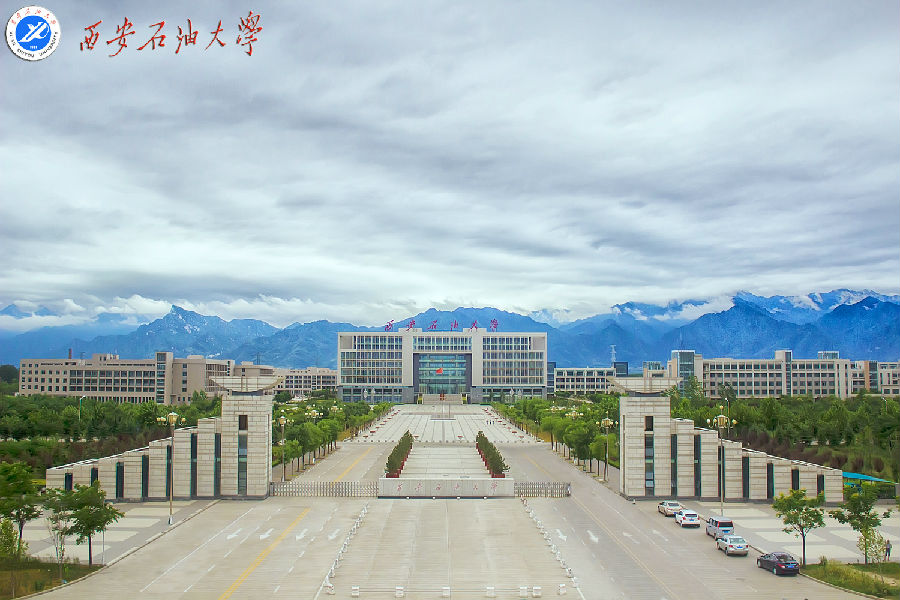
\includegraphics{figures/XSYU-birdview.jpg}
		}
		%\includegraphics[scale=1.0]{figurefile}
		\caption{鄠邑校区北门}
		\label{fig:campus}
	\end{figure}
\end{column}%
\hfill%
\begin{column}<0->{.65\textwidth}
	\begin{itemize}
		\item<1-> 鄠邑校区简介
		\begin{itemize}
			\item<1-> 位于西安市沣京工业园沣京大道18号。
		\end{itemize}
		\item<2-> 雁塔校区简介
		\begin{itemize}
			\item<2-> 位于西安市电子二路东段18号。
		\end{itemize}
	\end{itemize}
\end{column}%
\end{columns}
\end{frame}
\subsection{居中布局}
\begin{frame}
	\frametitle{居中布局}
	\begin{figure}[!t]
		\centering
		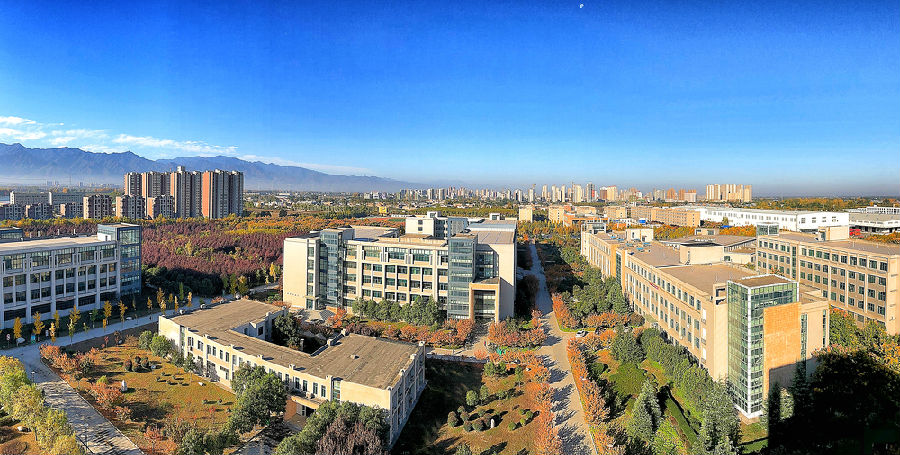
\includegraphics[width=2in]{figures/XSYU-autumn.jpg}
		\caption{校园秋色}
		\label{figure_autumn}
	\end{figure}
	\begin{center}
		计算机学院成立于2003年5月\footfullcite[1]{zhang}。\\
		学院现设有计算机科学与技术系、软件工程系、数字媒体系、通信工程系、网络工程系、数据科学与大数据技术系、计算机基础部、实验教学示范中心和培训部。
	\end{center}
	\end{frame}
\section{文本块}
\begin{frame}{文本块}
本模板提供三种文本色块如下:
\begin{block}{block}
		block常用于一般描述
	\end{block}
\begin{exampleblock}{exampleblock}
	exampleblock常用于举例
\end{exampleblock}
\begin{alertblock}{Alert block}
	alert block常用于强调
\end{alertblock}
\end{frame}

\section{双栏}
\begin{frame}{双栏}
\begin{columns}[c] % align columns
	\begin{column}<0->{.4\textwidth}
		左栏
		\begin{block}{block}
			左栏中可以混排文本块
		\end{block}
    \end{column}%
\hfill%	
	\begin{column}<0->{.4\textwidth}
		右栏
		\begin{block}{block}
			右栏中可以混排文本块
		\end{block}
    \end{column}%
\end{columns}
\end{frame}

\section{混合排版}  
\begin{frame}{计算机视觉任务}
	计算机视觉是关于研究机器视觉能力的学科,或者说是使机器能对环境和其中的刺激进行可视化分析的学科。机器视觉通常涉及对图像或视频的评估,英国机器视觉协会(BMVA)将机器视觉定义为“对单张图像或一系列图像的有用信息进行自动提取、分析和理解”。
\begin{block}{主要任务}
	图像分类(Image Classification)
	\begin{itemize}
		\item<0-> 在分类任务中,CNN经典神经网络结构是AlexNet网络模型
	\end{itemize}
	目标检测(Object Dection)
	\begin{itemize}
		\item<0-> R-CNN
		\item<0-> Fast R-CNN
		\item<0-> YOLO、SSD以及R-FCN
	\end{itemize}
	图像定位等
\end{block}
\end{frame}

\begin{frame}{One-Hot Representation}
最简单直接的词表示是One-Hot Representation。考虑一个词表$ \mathbb V $,里面的每一个词$ w_i $都有一个编号$ i\in \{1,...,n\} $,那么词$ w_i $的one-hot表示就是一个维度为n的向量,其中第$ i $个元素值非零,其余元素全为0。例如:
\[  w_2=[0,1,0,...,0]^\top  \]
\[  w_3=[0,0,1,...,0]^\top  \]
\begin{block}{缺点}
	\begin{itemize}
		\item<0-> 彼此正交,不能反应词间的语义关系
		\item<0-> 稀疏表示,维度很高,和词典大小成正比
	\end{itemize}
\end{block}
\end{frame}

\section{字体颜色}
\begin{frame}{颜色展示}
	\textcolor{mygray}{让我们紧紧依靠在一起,倾听灵魂的声音,祈求内心风平浪静}\\
	\textcolor{mygreen}{让我们紧紧依靠在一起,倾听灵魂的声音,祈求内心风平浪静}\\
	\textcolor{mypink}{让我们紧紧依靠在一起,倾听灵魂的声音,祈求内心风平浪静}\\
	\textcolor{mycyan}{让我们紧紧依靠在一起,倾听灵魂的声音,祈求内心风平浪静}\\
	\textcolor{mymauve}{让我们紧紧依靠在一起,倾听灵魂的声音,祈求内心风平浪静}
\end{frame}
\section{利用Tikz包绘图}
\subsection{简单图形}
\begin{frame}{图例1}
	\begin{center}
		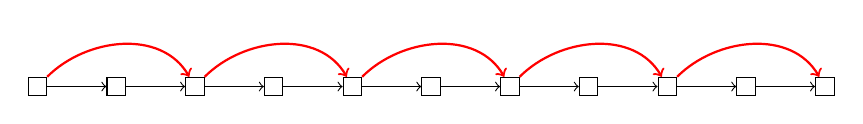
\begin{tikzpicture}
		\xdef\lastx{1}
		\node[draw=black] (1)  {};
		\foreach \x in {2,3,4,5,6,7,8,9,10,11} {
		\node[draw=black, right of=\lastx] (\x)  {~};
		\draw[->] (\lastx)--(\x);
		\xdef\lastx{\x}
		}
		\xdef\lastx{1}
		\foreach \x in {3,5,7,9,11} {
		\draw[->, thick, draw=red] (\lastx) to [out=45,in=120] (\x);
		\xdef\lastx{\x}
		}
		
		\end{tikzpicture}
		
		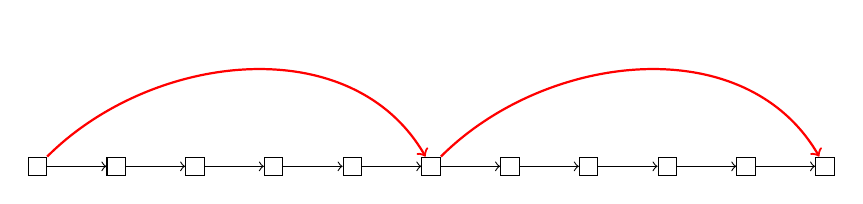
\begin{tikzpicture}
		\xdef\lastx{1}
		\node[draw=black] (1)  {};
		\foreach \x in {2,3,4,5,6,7,8,9,10,11} {
		\node[draw=black, right of=\lastx] (\x)  {~};
		\draw[->] (\lastx)--(\x);
		\xdef\lastx{\x}
		}
		\draw[->, thick, draw=red] (1) to [out=45,in=120] (6);
		\draw[->, thick, draw=red] (6) to [out=45,in=120] (11);
		\end{tikzpicture}
		\end{center}
\end{frame}
\subsection{复杂图}
\begin{frame}{神经网络}
	\begin{center}
	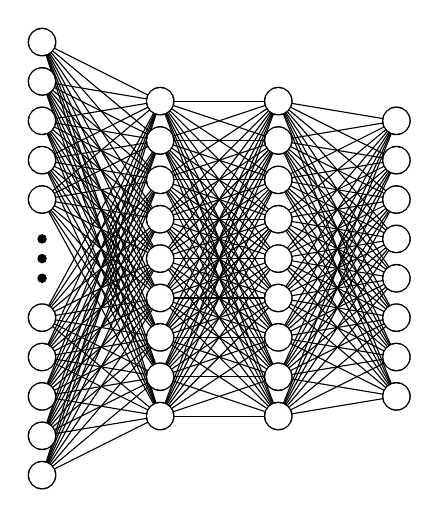
\begin{tikzpicture}[scale=0.5]
        %———————————————————————连线开始———————————————————————
        \draw [-] (0,-11) -- (3,-9.5);
        \draw [-] (0,-11) -- (3,-8.5);
        \draw [-] (0,-11) -- (3,-7.5);
        \draw [-] (0,-11) -- (3,-6.5);
        \draw [-] (0,-11) -- (3,-5.5);
        \draw [-] (0,-11) -- (3,-4.5);
        \draw [-] (0,-11) -- (3,-3.5);
        \draw [-] (0,-11) -- (3,-2.5);
        \draw [-] (0,-11) -- (3,-1.5);

        \draw [-] (0,-10) -- (3,-9.5);
        \draw [-] (0,-10) -- (3,-8.5);
        \draw [-] (0,-10) -- (3,-7.5);
        \draw [-] (0,-10) -- (3,-6.5);
        \draw [-] (0,-10) -- (3,-5.5);
        \draw [-] (0,-10) -- (3,-4.5);
        \draw [-] (0,-10) -- (3,-3.5);
        \draw [-] (0,-10) -- (3,-2.5);
        \draw [-] (0,-10) -- (3,-1.5);

        \draw [-] (0,-9) -- (3,-9.5);
        \draw [-] (0,-9) -- (3,-8.5);
        \draw [-] (0,-9) -- (3,-7.5);
        \draw [-] (0,-9) -- (3,-6.5);
        \draw [-] (0,-9) -- (3,-5.5);
        \draw [-] (0,-9) -- (3,-4.5);
        \draw [-] (0,-9) -- (3,-3.5);
        \draw [-] (0,-9) -- (3,-2.5);
        \draw [-] (0,-9) -- (3,-1.5);

        \draw [-] (0,-8) -- (3,-9.5);
        \draw [-] (0,-8) -- (3,-8.5);
        \draw [-] (0,-8) -- (3,-7.5);
        \draw [-] (0,-8) -- (3,-6.5);
        \draw [-] (0,-8) -- (3,-5.5);
        \draw [-] (0,-8) -- (3,-4.5);
        \draw [-] (0,-8) -- (3,-3.5);
        \draw [-] (0,-8) -- (3,-2.5);
        \draw [-] (0,-8) -- (3,-1.5);

        \draw [-] (0,-7) -- (3,-9.5);
        \draw [-] (0,-7) -- (3,-8.5);
        \draw [-] (0,-7) -- (3,-7.5);
        \draw [-] (0,-7) -- (3,-6.5);
        \draw [-] (0,-7) -- (3,-5.5);
        \draw [-] (0,-7) -- (3,-4.5);
        \draw [-] (0,-7) -- (3,-3.5);
        \draw [-] (0,-7) -- (3,-2.5);
        \draw [-] (0,-7) -- (3,-1.5);



        \draw [-] (0,-4) -- (3,-9.5);
        \draw [-] (0,-4) -- (3,-8.5);
        \draw [-] (0,-4) -- (3,-7.5);
        \draw [-] (0,-4) -- (3,-6.5);
        \draw [-] (0,-4) -- (3,-5.5);
        \draw [-] (0,-4) -- (3,-4.5);
        \draw [-] (0,-4) -- (3,-3.5);
        \draw [-] (0,-4) -- (3,-2.5);
        \draw [-] (0,-4) -- (3,-1.5);

        \draw [-] (0,-3) -- (3,-9.5);
        \draw [-] (0,-3) -- (3,-8.5);
        \draw [-] (0,-3) -- (3,-7.5);
        \draw [-] (0,-3) -- (3,-6.5);
        \draw [-] (0,-3) -- (3,-5.5);
        \draw [-] (0,-3) -- (3,-4.5);
        \draw [-] (0,-3) -- (3,-3.5);
        \draw [-] (0,-3) -- (3,-2.5);
        \draw [-] (0,-3) -- (3,-1.5);

        \draw [-] (0,-2) -- (3,-9.5);
        \draw [-] (0,-2) -- (3,-8.5);
        \draw [-] (0,-2) -- (3,-7.5);
        \draw [-] (0,-2) -- (3,-6.5);
        \draw [-] (0,-2) -- (3,-5.5);
        \draw [-] (0,-2) -- (3,-4.5);
        \draw [-] (0,-2) -- (3,-3.5);
        \draw [-] (0,-2) -- (3,-2.5);
        \draw [-] (0,-2) -- (3,-1.5);

        \draw [-] (0,-1) -- (3,-9.5);
        \draw [-] (0,-1) -- (3,-8.5);
        \draw [-] (0,-1) -- (3,-7.5);
        \draw [-] (0,-1) -- (3,-6.5);
        \draw [-] (0,-1) -- (3,-5.5);
        \draw [-] (0,-1) -- (3,-4.5);
        \draw [-] (0,-1) -- (3,-3.5);
        \draw [-] (0,-1) -- (3,-2.5);
        \draw [-] (0,-1) -- (3,-1.5);

        \draw [-] (0,0) -- (3,-9.5);
        \draw [-] (0,0) -- (3,-8.5);
        \draw [-] (0,0) -- (3,-7.5);
        \draw [-] (0,0) -- (3,-6.5);
        \draw [-] (0,0) -- (3,-5.5);
        \draw [-] (0,0) -- (3,-4.5);
        \draw [-] (0,0) -- (3,-3.5);
        \draw [-] (0,0) -- (3,-2.5);
        \draw [-] (0,0) -- (3,-1.5);


        \draw [-] (3,-9.5) -- (6,-9.5);
        \draw [-] (3,-8.5) -- (6,-9.5);
        \draw [-] (3,-7.5) -- (6,-9.5);
        \draw [-] (3,-6.5) -- (6,-9.5);
        \draw [-] (3,-5.5) -- (6,-9.5);
        \draw [-] (3,-4.5) -- (6,-9.5);
        \draw [-] (3,-3.5) -- (6,-9.5);
        \draw [-] (3,-2.5) -- (6,-9.5);
        \draw [-] (3,-1.5) -- (6,-9.5);

        \draw [-] (3,-9.5) -- (6,-8.5);
        \draw [-] (3,-8.5) -- (6,-8.5);
        \draw [-] (3,-7.5) -- (6,-8.5);
        \draw [-] (3,-6.5) -- (6,-8.5);
        \draw [-] (3,-5.5) -- (6,-8.5);
        \draw [-] (3,-4.5) -- (6,-8.5);
        \draw [-] (3,-3.5) -- (6,-8.5);
        \draw [-] (3,-2.5) -- (6,-8.5);
        \draw [-] (3,-1.5) -- (6,-8.5);

        \draw [-] (3,-9.5) -- (6,-7.5);
        \draw [-] (3,-8.5) -- (6,-7.5);
        \draw [-] (3,-7.5) -- (6,-7.5);
        \draw [-] (3,-6.5) -- (6,-7.5);
        \draw [-] (3,-5.5) -- (6,-7.5);
        \draw [-] (3,-4.5) -- (6,-7.5);
        \draw [-] (3,-3.5) -- (6,-7.5);
        \draw [-] (3,-2.5) -- (6,-7.5);
        \draw [-] (3,-1.5) -- (6,-7.5);

        \draw [-] (3,-9.5) -- (6,-6.5);
        \draw [-] (3,-8.5) -- (6,-6.5);
        \draw [-] (3,-7.5) -- (6,-6.5);
        \draw [-] (3,-6.5) -- (6,-6.5);
        \draw [-] (3,-5.5) -- (6,-6.5);
        \draw [-] (3,-4.5) -- (6,-6.5);
        \draw [-] (3,-3.5) -- (6,-6.5);
        \draw [-] (3,-2.5) -- (6,-6.5);
        \draw [-] (3,-1.5) -- (6,-6.5);

        \draw [-] (3,-9.5) -- (6,-5.5);
        \draw [-] (3,-8.5) -- (6,-5.5);
        \draw [-] (3,-7.5) -- (6,-5.5);
        \draw [-] (3,-6.5) -- (6,-5.5);
        \draw [-] (3,-5.5) -- (6,-5.5);
        \draw [-] (3,-4.5) -- (6,-5.5);
        \draw [-] (3,-3.5) -- (6,-5.5);
        \draw [-] (3,-2.5) -- (6,-5.5);
        \draw [-] (3,-1.5) -- (6,-5.5);

        \draw [-] (3,-9.5) -- (6,-4.5);
        \draw [-] (3,-8.5) -- (6,-4.5);
        \draw [-] (3,-7.5) -- (6,-4.5);
        \draw [-] (3,-6.5) -- (6,-4.5);
        \draw [-] (3,-5.5) -- (6,-4.5);
        \draw [-] (3,-4.5) -- (6,-4.5);
        \draw [-] (3,-3.5) -- (6,-4.5);
        \draw [-] (3,-2.5) -- (6,-4.5);
        \draw [-] (3,-1.5) -- (6,-4.5);

        \draw [-] (3,-9.5) -- (6,-3.5);
        \draw [-] (3,-8.5) -- (6,-3.5);
        \draw [-] (3,-7.5) -- (6,-3.5);
        \draw [-] (3,-6.5) -- (6,-3.5);
        \draw [-] (3,-5.5) -- (6,-3.5);
        \draw [-] (3,-4.5) -- (6,-3.5);
        \draw [-] (3,-3.5) -- (6,-3.5);
        \draw [-] (3,-2.5) -- (6,-3.5);
        \draw [-] (3,-1.5) -- (6,-3.5);

        \draw [-] (3,-9.5) -- (6,-2.5);
        \draw [-] (3,-8.5) -- (6,-2.5);
        \draw [-] (3,-7.5) -- (6,-2.5);
        \draw [-] (3,-6.5) -- (6,-2.5);
        \draw [-] (3,-5.5) -- (6,-2.5);
        \draw [-] (3,-4.5) -- (6,-2.5);
        \draw [-] (3,-3.5) -- (6,-2.5);
        \draw [-] (3,-2.5) -- (6,-2.5);
        \draw [-] (3,-1.5) -- (6,-2.5);

        \draw [-] (3,-9.5) -- (6,-1.5);
        \draw [-] (3,-8.5) -- (6,-1.5);
        \draw [-] (3,-7.5) -- (6,-1.5);
        \draw [-] (3,-6.5) -- (6,-1.5);
        \draw [-] (3,-5.5) -- (6,-1.5);
        \draw [-] (3,-4.5) -- (6,-1.5);
        \draw [-] (3,-3.5) -- (6,-1.5);
        \draw [-] (3,-2.5) -- (6,-1.5);
        \draw [-] (3,-1.5) -- (6,-1.5);




        \draw [-] (9,-9) -- (6,-1.5);
        \draw [-] (9,-8) -- (6,-1.5);
        \draw [-] (9,-7) -- (6,-1.5);
        \draw [-] (9,-6) -- (6,-1.5);
        \draw [-] (9,-5) -- (6,-1.5);
        \draw [-] (9,-4) -- (6,-1.5);
        \draw [-] (9,-3) -- (6,-1.5);
        \draw [-] (9,-2) -- (6,-1.5);

        \draw [-] (9,-9) -- (6,-2.5);
        \draw [-] (9,-8) -- (6,-2.5);
        \draw [-] (9,-7) -- (6,-2.5);
        \draw [-] (9,-6) -- (6,-2.5);
        \draw [-] (9,-5) -- (6,-2.5);
        \draw [-] (9,-4) -- (6,-2.5);
        \draw [-] (9,-3) -- (6,-2.5);
        \draw [-] (9,-2) -- (6,-2.5);

        \draw [-] (9,-9) -- (6,-3.5);
        \draw [-] (9,-8) -- (6,-3.5);
        \draw [-] (9,-7) -- (6,-3.5);
        \draw [-] (9,-6) -- (6,-3.5);
        \draw [-] (9,-5) -- (6,-3.5);
        \draw [-] (9,-4) -- (6,-3.5);
        \draw [-] (9,-3) -- (6,-3.5);
        \draw [-] (9,-2) -- (6,-3.5);

        \draw [-] (9,-9) -- (6,-4.5);
        \draw [-] (9,-8) -- (6,-4.5);
        \draw [-] (9,-7) -- (6,-4.5);
        \draw [-] (9,-6) -- (6,-4.5);
        \draw [-] (9,-5) -- (6,-4.5);
        \draw [-] (9,-4) -- (6,-4.5);
        \draw [-] (9,-3) -- (6,-4.5);
        \draw [-] (9,-2) -- (6,-4.5);

        \draw [-] (9,-9) -- (6,-5.5);
        \draw [-] (9,-8) -- (6,-5.5);
        \draw [-] (9,-7) -- (6,-5.5);
        \draw [-] (9,-6) -- (6,-5.5);
        \draw [-] (9,-5) -- (6,-5.5);
        \draw [-] (9,-4) -- (6,-5.5);
        \draw [-] (9,-3) -- (6,-5.5);
        \draw [-] (9,-2) -- (6,-5.5);

        \draw [-] (9,-9) -- (6,-6.5);
        \draw [-] (9,-8) -- (6,-6.5);
        \draw [-] (9,-7) -- (6,-6.5);
        \draw [-] (9,-6) -- (6,-6.5);
        \draw [-] (9,-5) -- (6,-6.5);
        \draw [-] (9,-4) -- (6,-6.5);
        \draw [-] (9,-3) -- (6,-6.5);
        \draw [-] (9,-2) -- (6,-6.5);

        \draw [-] (9,-9) -- (6,-7.5);
        \draw [-] (9,-8) -- (6,-7.5);
        \draw [-] (9,-7) -- (6,-7.5);
        \draw [-] (9,-6) -- (6,-7.5);
        \draw [-] (9,-5) -- (6,-7.5);
        \draw [-] (9,-4) -- (6,-7.5);
        \draw [-] (9,-3) -- (6,-7.5);
        \draw [-] (9,-2) -- (6,-7.5);

        \draw [-] (9,-9) -- (6,-8.5);
        \draw [-] (9,-8) -- (6,-8.5);
        \draw [-] (9,-7) -- (6,-8.5);
        \draw [-] (9,-6) -- (6,-8.5);
        \draw [-] (9,-5) -- (6,-8.5);
        \draw [-] (9,-4) -- (6,-8.5);
        \draw [-] (9,-3) -- (6,-8.5);
        \draw [-] (9,-2) -- (6,-8.5);

        \draw [-] (9,-9) -- (6,-9.5);
        \draw [-] (9,-8) -- (6,-9.5);
        \draw [-] (9,-7) -- (6,-9.5);
        \draw [-] (9,-6) -- (6,-9.5);
        \draw [-] (9,-5) -- (6,-9.5);
        \draw [-] (9,-4) -- (6,-9.5);
        \draw [-] (9,-3) -- (6,-9.5);
        \draw [-] (9,-2) -- (6,-9.5);

        %———————————————————————第一列开始———————————————————————
        \filldraw [black] (0,0) circle [radius=10pt];
        \filldraw [white] (0,0) circle [radius=9pt];

        \filldraw [black] (0,-1) circle [radius=10pt];
        \filldraw [white] (0,-1) circle [radius=9pt];

        \filldraw [black] (0,-2) circle [radius=10pt];
        \filldraw [white] (0,-2) circle [radius=9pt];

        \filldraw [black] (0,-3) circle [radius=10pt];
        \filldraw [white] (0,-3) circle [radius=9pt];

        \filldraw [black] (0,-4) circle [radius=10pt];
        \filldraw [white] (0,-4) circle [radius=9pt];

        \filldraw [black] (0,-5) circle [radius=3pt];

        \filldraw [black] (0,-5.5) circle [radius=3pt];

        \filldraw [black] (0,-6) circle [radius=3pt];

        \filldraw [black] (0,-7) circle [radius=10pt];
        \filldraw [white] (0,-7) circle [radius=9pt];

        \filldraw [black] (0,-8) circle [radius=10pt];
        \filldraw [white] (0,-8) circle [radius=9pt];

        \filldraw [black] (0,-9) circle [radius=10pt];
        \filldraw [white] (0,-9) circle [radius=9pt];

        \filldraw [black] (0,-10) circle [radius=10pt];
        \filldraw [white] (0,-10) circle [radius=9pt];

        \filldraw [black] (0,-11) circle [radius=10pt];
        \filldraw [white] (0,-11) circle [radius=9pt];

        %———————————————————————第一列结束———————————————————————

        %———————————————————————第二列开始———————————————————————

        \filldraw [black] (3,-1.5) circle [radius=10pt];
        \filldraw [white] (3,-1.5) circle [radius=9pt];

        \filldraw [black] (3,-2.5) circle [radius=10pt];
        \filldraw [white] (3,-2.5) circle [radius=9pt];

        \filldraw [black] (3,-3.5) circle [radius=10pt];
        \filldraw [white] (3,-3.5) circle [radius=9pt];

        \filldraw [black] (3,-4.5) circle [radius=10pt];
        \filldraw [white] (3,-4.5) circle [radius=9pt];

        \filldraw [black] (3,-5.5) circle [radius=10pt];
        \filldraw [white] (3,-5.5) circle [radius=9pt];

        \filldraw [black] (3,-6.5) circle [radius=10pt];
        \filldraw [white] (3,-6.5) circle [radius=9pt];

        \filldraw [black] (3,-7.5) circle [radius=10pt];
        \filldraw [white] (3,-7.5) circle [radius=9pt];

        \filldraw [black] (3,-8.5) circle [radius=10pt];
        \filldraw [white] (3,-8.5) circle [radius=9pt];

        \filldraw [black] (3,-9.5) circle [radius=10pt];
        \filldraw [white] (3,-9.5) circle [radius=9pt];

        %———————————————————————第二列结束———————————————————————

        %———————————————————————第三列开始———————————————————————

        \filldraw [black] (6,-1.5) circle [radius=10pt];
        \filldraw [white] (6,-1.5) circle [radius=9pt];

        \filldraw [black] (6,-2.5) circle [radius=10pt];
        \filldraw [white] (6,-2.5) circle [radius=9pt];

        \filldraw [black] (6,-3.5) circle [radius=10pt];
        \filldraw [white] (6,-3.5) circle [radius=9pt];

        \filldraw [black] (6,-4.5) circle [radius=10pt];
        \filldraw [white] (6,-4.5) circle [radius=9pt];

        \filldraw [black] (6,-5.5) circle [radius=10pt];
        \filldraw [white] (6,-5.5) circle [radius=9pt];

        \filldraw [black] (6,-6.5) circle [radius=10pt];
        \filldraw [white] (6,-6.5) circle [radius=9pt];

        \filldraw [black] (6,-7.5) circle [radius=10pt];
        \filldraw [white] (6,-7.5) circle [radius=9pt];

        \filldraw [black] (6,-8.5) circle [radius=10pt];
        \filldraw [white] (6,-8.5) circle [radius=9pt];

        \filldraw [black] (6,-9.5) circle [radius=10pt];
        \filldraw [white] (6,-9.5) circle [radius=9pt];

        %———————————————————————第三列结束———————————————————————

        %———————————————————————第四列开始———————————————————————

        \filldraw [black] (9,-2) circle [radius=10pt];
        \filldraw [white] (9,-2) circle [radius=9pt];

        \filldraw [black] (9,-3) circle [radius=10pt];
        \filldraw [white] (9,-3) circle [radius=9pt];

        \filldraw [black] (9,-4) circle [radius=10pt];
        \filldraw [white] (9,-4) circle [radius=9pt];

        \filldraw [black] (9,-5) circle [radius=10pt];
        \filldraw [white] (9,-5) circle [radius=9pt];

        \filldraw [black] (9,-6) circle [radius=10pt];
        \filldraw [white] (9,-6) circle [radius=9pt];

        \filldraw [black] (9,-7) circle [radius=10pt];
        \filldraw [white] (9,-7) circle [radius=9pt];

        \filldraw [black] (9,-8) circle [radius=10pt];
        \filldraw [white] (9,-8) circle [radius=9pt];

        \filldraw [black] (9,-9) circle [radius=10pt];
        \filldraw [white] (9,-9) circle [radius=9pt];

        %———————————————————————第四列结束———————————————————————
    \end{tikzpicture}
\end{center}
\end{frame}
\begin{frame}{流程图}
% 流程图定义基本形状
\tikzstyle{startstop} = [rectangle, rounded corners, minimum width = 2cm, minimum height=1cm,text centered, draw = black, fill = red!40]
\tikzstyle{io} = [trapezium, trapezium left angle=70, trapezium right angle=110, minimum width=2cm, minimum height=1cm, text centered, draw=black, fill = blue!40]
\tikzstyle{process} = [rectangle, minimum width=3cm, minimum height=1cm, text centered, draw=black, fill = yellow!50]
\tikzstyle{decision} = [diamond, aspect = 3, text centered, draw=black, fill = green!30]
% 箭头形式
\tikzstyle{arrow} = [->,>=stealth]
\tikzstyle{every node}=[font=\small,scale=0.6]
\centering
\begin{tikzpicture}[node distance=1.5cm]
%定义流程图具体形状
\node (start) [startstop] {start};
\node (pro1) [process, below of=start, yshift=-0.2cm, left of=start, xshift=-1cm] {PROCESS 1};
\node (pro2) [process, right of=pro1, xshift= 4cm] {PROCESS 2};
\node (in1) [io, below of=pro1, yshift= -0.2cm, right of=pro1, xshift=1cm] {IO};
\node (pro3) [process, below of=in1, yshift= -0.2cm] {PROCESS 3};
\node (in2) [io, below of=pro3, yshift= -0.2cm] {IO 2};
\node (dec1) [decision, below of=in2, yshift= -0.2cm] {DECISION};
\node (stop) [startstop, below of=dec1] {end};

%连接具体形状
\draw [arrow](start) -- (pro1);
\draw [arrow](start) -- (pro2);
\draw [arrow](pro1) -- (in1);
\draw [arrow](pro2) -- (in1);
\draw [arrow](in1) -- (pro3);
\draw [arrow](pro3) -- (in2);
\draw [arrow](in2) -- (dec1);
\draw [arrow](dec1) -- ($(dec1.east) + (1.5,0)$) node[anchor=north] {NO} |- (pro3);
\draw [arrow](dec1) -- node[anchor=west] {YES} (stop);
\end{tikzpicture}
\end{frame}
\section{表格和公式}
\subsection{表格}
\begin{frame}{研究方法与数据集特征}
\begin{columns}[c] % align columns
	\begin{column}<0->{.4\textwidth}
		\begin{table}\footnotesize
			% table caption is above the table
			\caption{三线表}
			\label{tab:1}       % Give a unique label
			% For LaTeX tables use
			\begin{tabular}{lll}
			\hline\noalign{\smallskip}
			first & second & third  \\
			\noalign{\smallskip}\hline\noalign{\smallskip}
			number & number & number \\
			number & number & number \\
			\noalign{\smallskip}\hline
			\end{tabular}
			\end{table}
    \end{column}%
\hfill%	
	\begin{column}<0->{.6\textwidth}
		\begin{table}
			\caption{带颜色表格}
			\footnotesize
			\rowcolors{1}{mygray}{white}
			\begin{tabular}{|c|c|}
				\hline
				\textbf{Site}           & \textbf{Messages}\\
				\hline
				receivesmsonline.net    &81313\\
				\hline
				receive-sms-online.info &69389\\
				\hline
				receive-sms-now.com     &63797\\
				\hline
				hs3x.com               &55499\\
				\hline
				receivesmsonline.com    &44640\\
				\hline
				receivefreesms.com      &37485\\
				\hline
				receive-sms-online.com  &27094\\
				\hline
				e-receivesms.com       &7107\\
				\hline
			\end{tabular}
		\end{table}
    \end{column}%
\end{columns}
\end{frame}
\subsection{公式}
\begin{frame}{公式}
	行内公式是这样的$ f(x) = a+b $。\\
	行间公式如下:
	$$  \lim_{x \to \infty} x^2_{22} - \int_{1}^{5}x\mathrm{d}x + \sum_{n=1}^{20} n^{2} = \prod_{j=1}^{3} y_{j}  + \lim_{x \to -2} \frac{x-2}{x} $$
\end{frame}

\section{算法和代码}
\subsection{算法}
\begin{frame}{算法}
\begin{algorithm}[H]
	\caption{HOSVD}
	\small 
	\KwIn{HOSVD($\mathcal{X},R_{1},R_{2}.....R_{N}$) }
	\KwOut{ $\mathcal{G},A_{(1)},A_{(2)}......A_{(N)} $ }
	
	\For{$k=1$ to $N$ }
	{
		$A_{(n)}\leftarrow R_{n}$left singular matrix of $X_{(n)}$
	}
	$\mathcal{G}=\leftarrow \mathcal{X} \times A_{(1)}^{T} \times A_{(2)}^{T}...... \times A_{(N)}^{T}$\\
	\Return $\mathcal{G},A_{(1)},A_{(2)}......A_{(N)} $
\end{algorithm}
\end{frame}

\subsection{代码}
\begin{frame}[fragile]{代码}
HOSVD在Python的代码实现和分析:
\lstinputlisting[lastline=11,
language=Python,
frame=single,
caption=First ten lines of some Python code,
label=python]
{HOSVD.py}
\end{frame}

\section{致谢和提问}
\begin{frame}{致谢}
\begin{center}
\begin{minipage}{1\textwidth}
	\setbeamercolor{mybox}{fg=white, bg=black!50!blue}
 \begin{beamercolorbox}[wd=0.70\textwidth, rounded=true, shadow=true]{mybox}
\LARGE \centering 感谢您的倾听!  %结束语
\end{beamercolorbox}
 \end{minipage}
\end{center}
\begin{alertblock}{注意用词}
	\begin{itemize}
		\item<0-> 倾听:指细心地听取,表示中性的感情色彩,就是凭借听觉器官接受言语信息,进而通过思维活动达到认知、理解的全过程。一般指上级对下级 ,表示上级听取下级的意见、报告等。
		\item<0-> 聆听:指虔诚而认真地听取,带有尊敬的色彩,一般多用于教诲、报告、演讲、讲学、朗诵、故事等有关人的活动,也可用于具体的事物。
	\end{itemize}
\end{alertblock}
\end{frame}

\begin{frame}{Q\&A}
\begin{center}
	\begin{minipage}{1\textwidth}
		\setbeamercolor{mybox}{fg=white, bg=black!50!blue}
		\begin{beamercolorbox}[wd=0.70\textwidth, rounded=true, shadow=true]{mybox}
			\LARGE \centering  请专家批评指正?  %请求提问
		\end{beamercolorbox}
	\end{minipage}
\end{center}
\end{frame}
\begin{frame}{参考文献}
	\printbibliography
\end{frame}
% -----------------------------------------------------------------------------
\end{document}
%文档结束